\documentclass[tikz,border=3.14mm]{standalone}
\usetikzlibrary{positioning}

\begin{document}
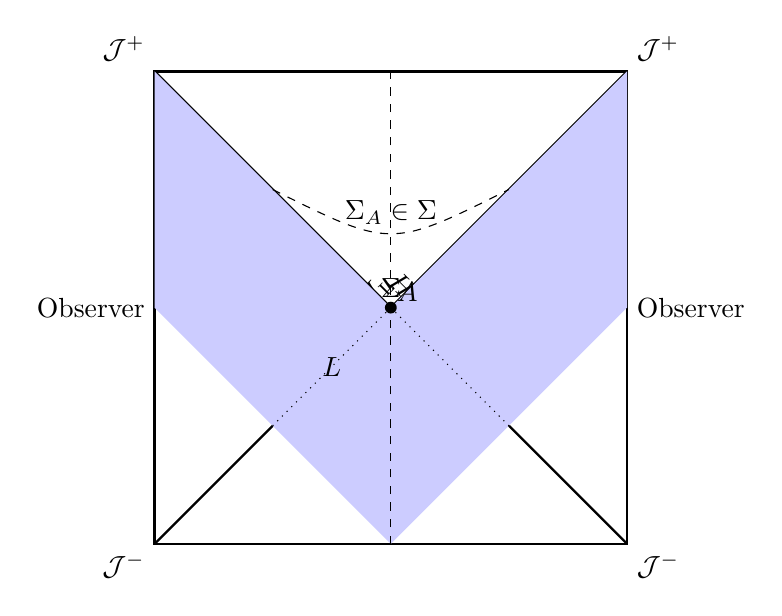
\begin{tikzpicture}[scale=1.5]
    % Diagram background
    \draw[thick] (0,0) -- (4,0) -- (4,4) -- (0,4) -- cycle;
    
    % Diagonal lines (cosmological horizons)
    \draw[thick] (0,4) -- (4,0) node[midway, sloped, above] {$H_{\rm R}$};
    \draw[thick] (0,0) -- (4,4) node[midway, sloped, above] {$H_{\rm L}$};
    
    % Static patches (blue shaded regions)
    \fill[blue!20] (0,2) -- (2,0) -- (2,2) -- (0,4) -- cycle; % P_L
    \fill[blue!20] (4,2) -- (2,0) -- (2,2) -- (4,4) -- cycle; % P_R
    
    % Observers
    \node at (0,2) [left] {Observer};
    \node at (4,2) [right] {Observer};
    
    % Light cones or boundaries (if needed, though not explicitly in description)
    \draw[dashed] (2,0) -- (2,4) node[midway, above] {$\Sigma$};
    
    % Arbitrary global spacelike slice (dashed line)
    \draw[dashed] (1,3) .. controls (2,2.5) .. (3,3) node[midway, above] {$\Sigma_A\in\Sigma$};
    
    % Sphere A (black dot)
    \fill (2,2) circle (0.05) node[above right, inner sep=2pt] {$A$};
    
    % Future lightsheet (dotted line)
    \draw[dotted] (2,2) -- (1,1);
    \draw[dotted] (2,2) -- (3,1);
    
    % Labels for lightsheets (optional, if needed)
    \node at (1.5,1.5) {$L$}; % If needed, can be adjusted or removed
    
    % Boundary labels
    \node at (0,4) [above left] {$\mathcal{J}^+$};
    \node at (0,0) [below left] {$\mathcal{J}^-$};
    \node at (4,4) [above right] {$\mathcal{J}^+$};
    \node at (4,0) [below right] {$\mathcal{J}^-$};
\end{tikzpicture}
\end{document}